\section{Introduction}
        L'objectif de ce projet est de réaliser un jeu vidéo massivement multijoueur sur navigateur. Celui ci se joue de deux façons bien distinctes :
        \begin{itemize}
            \item \textit{Mode "Péon"} : Le joueur contrôle un personnage et s'occupe des actions élémentaires telles que récupérer des ressources, construire des bâtiments, etc.
            \item \textit{Mode "Seigneur"} : Le joueur ne contrôle pas de personnage directement, mais a une vision plus globale et donne des ordres aux péons en fonction des besoins du royaume.
        \end{itemize}
        Il y aurait plusieurs royaumes gérés par des seigneurs différents, en concurrence pour devenir le royaume le plus puissant. L'idée est inspirée de la "pixel war", l'événement temporaire sur r/place de Reddit où tous les utilisateurs du site pouvaient dessiner sur une page blanche. Ce principe très simple avait créé des dynamiques de groupes autour de communautés d'Internet et de streamers notamment qui voulaient leur place sur ce tableau géant, et nous avions assisté à des guerres d'alliances et des trahisons. Là où le but de la pixel war était purement esthétique, notre jeu serait plus concurrentiel. L'objectif de notre projet est de recréer ces dynamiques de groupes dans les royaumes.

        %image pixelwar (long a charger)
        %\begin{figure}[!h]
        %   \centering
        %    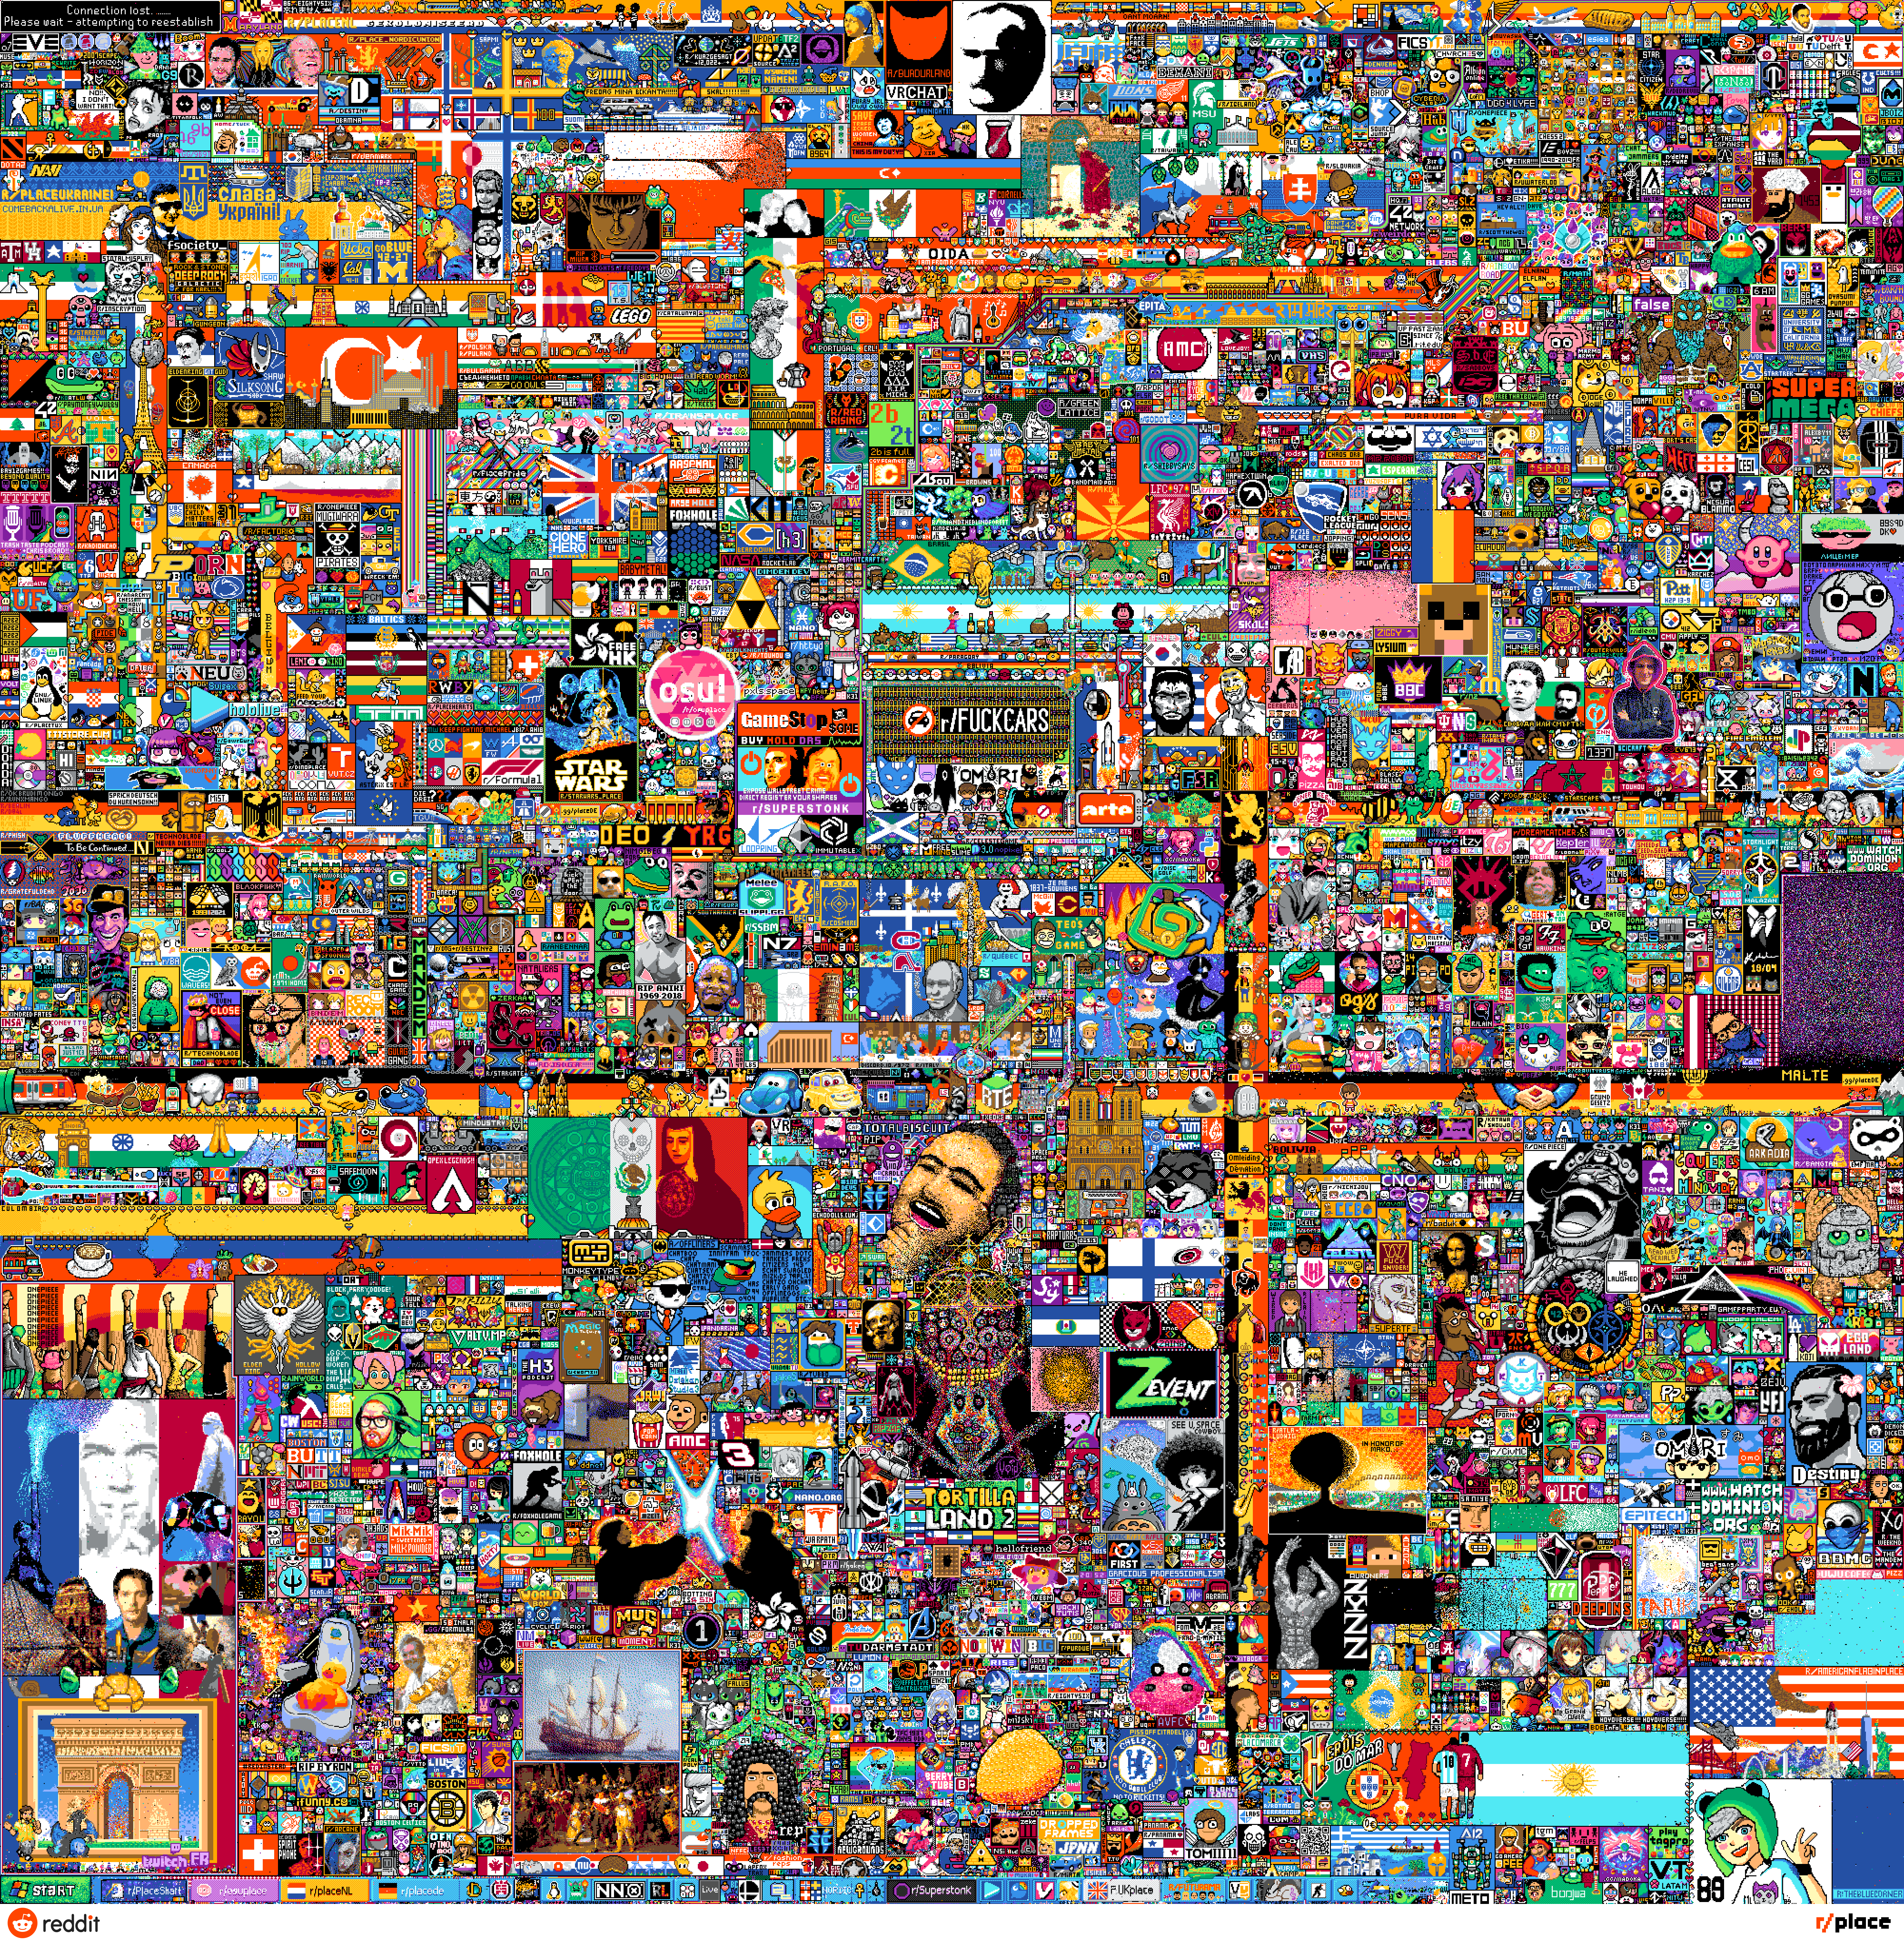
\includegraphics[width=0.5\linewidth]{images/pixelwar.png}
        %    \caption{Image finale de r/Place}
        %    \label{fig:enter-label}
        %\end{figure}